\documentclass[letterpaper, reqno,11pt]{article}
\usepackage[margin=1.0in]{geometry}
\usepackage{color,latexsym,amsmath,amssymb,graphicx,float,listings,tikz}
\usepackage{hyperref}

\hypersetup{
colorlinks=true,
linkcolor=magenta,
filecolor=magenta,
urlcolor=cyan,
}

\graphicspath{ {images/} }

\begin{document}
\pagenumbering{arabic}
\title{Math 318 Homework 8}
\date{23/03/23}
\author{Xander Naumenko}
\maketitle

{\medskip\noindent\bf Question 1a.} Let $T_i$ be the number of steps required to return to $0$ from a starting value of $i$ for standard random walk ($p=0.5$ with no chance of repeat), call this walk $w$. Similarly let $T'_i$ be the number of steps required to return from starting value $2i$ in the given walk, here referred to as $w'$. Let $p$ be the probability that the given random walk goes up or down, so $1-p$ is the probability that the walk stays at the same value. 

Since the magnitude of $w'$ is always exactly twice that of the corresponding state of $w$ and the target state is 0 which is unaffected by scaling, the fact that $w'$ jumps by 2 instead of 1 doesn't affect its recurrence. For a given state $i$, the expected number of times it repeats in $w'$ before going either up or down has a finite expected value and time after will have probability $\frac{1}{2}$ of going up and $\frac{1}{2}$ of going down, so the $w'$ has the same asymptotic behavior as $w$. Since $w$ is recurrent then $w'$ must be as well.

% To show that the possibility of repeating also doesn't affect recurrence, not that with probability $p$, $w'$ acts like $w$, and with probability $1-p$ it makes no progress. Thus $E[T'_i]=\frac{E[T_i]}{p}$. Since $E[T_i]$ is finite for all $i$, $E[T'_i]$ must also be finite. Since $E[T'_i]<\infty$, $w'$ is recurrent as required (if there was a nonzero probability that $w'$ never returns, i.e. $T'_i=\infty$ then $E[T'_i]$ would also be infinite, so $E[T'_i]$ being finite implies that this isn't true).

{\medskip\noindent\bf Question 1b.} Let $Z_n=X_n-Y_n$. At each step there is probability $p^2+(1-p)^2$ that $Z_n$ doesn't move as $X_n$ and $Y_n$ stepped in opposite directions, and probability $p(1-p)$ to go either up by two and $p(1-p)$ to go down by two. $Z_n$ is exactly a walk as describe in part a of this question, so by that result $Z_n$ is recurrent. However each zero of $Z_n$ corresponds to a point where $X_n=Y_n$, so there are infinite many $n$ such that $X_n=Y_n$.

{\medskip\noindent\bf Question 2a.} This Markov Chain is reducible, as the states $2, 3$ and the state $4$ have no way in the transition to one another for example. The communicating classes are $\{1\} $, $\{2,3\} $, $\{4\} $ and $\{5\} $ by simple inspection of what states are reachable from one another. For each state: 

{\bf 1}: Transient, aperiodic.

{\bf 2}: Recurrent, periodic.

{\bf 3}: Recurrent, periodic.

{\bf 4}: Transient, aperiodic.

{\bf 5}: Recurrent, aperiodic.

{\medskip\noindent\bf Question 2b.} The system is irreducible, as every state is accessible from the others. For the same reason the only communicating class is $\{1, 2, 3, 4, 5\} $. The one branch at state 1 means that none of the states are periodic, and they are all recurrent since every state is part of the same communicating class.

{\medskip\noindent\bf Question 2c.} The system is irreducible, since there's a nonzero probability of going between any two states (specifically it's at least $p^{n}$, where $n$ is the taxicab distance between the two states). Thus the only communicating class is $\mathbb{Z}^{d}$. Recurrence depends on dimension, as proved in class the random walk in $d\in \{1,2\} $ is recurrent and it is transient otherwise. Every state is periodic with period 2, since it is necessary to leave the state an go back which always takes an even number of steps. 

{\medskip\noindent\bf Question 2d.} For the same reason as part c, this random walk is irreducible and the only communicating class is $\mathbb{Z}$. However every state is transient as we proved in class. Again for the same reason as c every state is periodic with period 2, since the transition probabilities don't affect the periodicity. 

{\medskip\noindent\bf Question 3a.} If Cleopatra has $m$ camels then she has $n-m$ horses, and she has probability $\frac{m}{n}$ to give away a camel and probability $\frac{n-m}{m}$ to give away a horse, and similarly she has a $\frac{n-m}{m}$ chance to receive a camel and a $\frac{m}{n}$ chance to receive a horse. The three possible next states from a given state $X_m$ are either $X_{m+1},X_{m}$ or $X_{m-1}$ with probabilities $\frac{(n-m)^2}{n^2}$, $\frac{2m(n-m)}{n^2}$ and $\frac{m^2}{n^2}$ respectively.

{\medskip\noindent\bf Question 3b.} Let $X_0=\pi$. The net change to a given state $i$ will come from the state above, below or staying the same. Thus: 
\[
    X_1\sim\frac{{n\choose i-1}^2}{{2n\choose n}}\frac{\left( n-i+1 \right)^2 }{n^2}+\frac{{n\choose i}^2}{{2n\choose n}}\frac{2i(n-i)}{n^2}+\frac{{n\choose i+1}^2}{{2n\choose n}}\frac{(i+1)^2}{n^2}
.\]
\[
    =\frac{n!^2}{{2n\choose n}}\frac{1}{n^2}\left( \frac{(n-i+1)^2}{(i-1)!^2(n-i+1)!^2}+\frac{2i(n-i)}{(n-i)!^2i!^2}+\frac{(i+1)^2}{(i+1)!^2(n-i-1)!^2} \right) 
.\]
\[
=\frac{{n\choose i}^2}{{2n\choose n}}\frac{1}{n^2}\left( i^2+2i(n-i)+(n-i-1)^2 \right)=\frac{{n\choose i}^2}{{2n\choose n}}\sim X_0
.\]

{\medskip\noindent\bf Question 4.} No matter what coin we pick, we have a $\frac{1}{2}$ chance to flip it to whatever it already was, so $P_{ii}=\frac{1}{2}$. The probability of choosing heads is $\frac{m}{n}$ and conditional on this there is a $\frac{1}{2} $ chance of getting tails, so $P_{i,i-1}=\frac{1}{2}\frac{i}{n}$. Similarly, there is a $\frac{n-m}{n}$ chance of picking a tails and from there a $\frac{1}{2}$ chance of flipping heads, so $P_{i,i+1}=\frac{1}{2}\frac{n-i}{n}$. These are exactly the transition probabilities that were given so we're done. 

{\noindent\bf Bonus:} I guess that the stationary distribution is the normal distribution, so assume that $\pi_i=\frac{1}{2^{n}}{n\choose i}$. We can verify using the same method we used in problem 3, where we let $X_0\sim \pi$ and compute $X_1$: 

\[
    X_1\sim \frac{1}{2}\frac{1}{2^{n}}{n\choose i}+\frac{i+1}{2n}\frac{1}{2^{n}}{n\choose i+1}+\frac{n-i+1}{2n}\frac{1}{2^{n}}{n\choose i-1}
.\]
\[
    =\frac{1}{2}\frac{1}{2^{n}}{n\choose i}+\frac{n-i}{2n}\frac{1}{2^{n}}{n\choose i}+\frac{i}{2n}\frac{1}{2^{n}}{n\choose i}=\frac{1}{2^{n}}{n\choose i}\sim X_0
.\]


{\medskip\noindent\bf Question 5a.} As the hint suggests, let $X=M_k$ and we have
\[
    EX=(1+E[X+1])p+(1+E[X-1])q=1+pE[X+1]+qE[X-1]\implies M_k=1+pM_{k+1}+qM_{k-1}
\]

{\medskip\noindent\bf Question 5b.} Guess $M_k=x^{k}$. We will solve the homogeneous equation
\[
x^{k}=px^{k+1}+qx^{k-1}\implies px^2-x+q=0\implies x=\frac{1}{2p}\pm \frac{\sqrt{1-4pq} }{2p}=1\text{ or }\frac{q}{p}
.\]

Next for the inhomogenous equation, as the hit suggests guess $M_k=ck^2$ for $p=1 /2$ and $M_k=ck$ for $p\neq 1 /2$:
\[
1+\frac{1}{2}c(k+1)^2+\frac{1}{2}c(k-1)^2=ck^2\implies c=-1
\]
\[
1+pc(k+1)+qc(k-1)=ck \implies qc-pc=1\implies c=\frac{1}{q-p}
.\]

Therefore applying the boundary conditions of $M_0=0$ and $M_n=0$ we get that we have that for $p=\frac{1}{2}$:
\[
M_k=-k^2+a\implies M_k=k(n-k)
.\]
Similarly for $p\neq 1 /2$:
\[
M_k=\frac{k}{q-p}+a+b\alpha^{k}\implies \frac{k}{q-p}-\frac{n}{q-p}\frac{1-\alpha ^{k}}{1-\alpha ^{n}}
.\]

{\medskip\noindent\bf Question 6.} The graph for $X_t$ can be seen in figure \ref{fig:q6a}. Similarly the other plots can be seen in figures \ref{fig:q6b}, \ref{fig:q6c} and \ref{fig:q6d}. The code used was: 

\begin{lstlisting}
import matplotlib.pyplot as plt
import random
import numpy as np
from collections import Counter


n = 1000
steps = 200000

X = [0]
for i in range(steps):
    newX = X[-1]
    if random.random() < X[-1] / n:
        newX-=1
    if random.random() < (n-X[-1]) / n:
        newX+=1
    X.append(newX)

plt.plot(X)
plt.show()
        
occur1 = Counter(X[:1000])
occur2 = Counter(X[1000:2000])
occur3 = Counter(X[10000:])

plt.bar(occur1.keys(), occur1.values())
plt.show()
plt.bar(occur2.keys(), occur2.values())
plt.show()
plt.bar(occur3.keys(), occur3.values())
plt.show()
\end{lstlisting}

\begin{figure}[htpb]
    \centering
    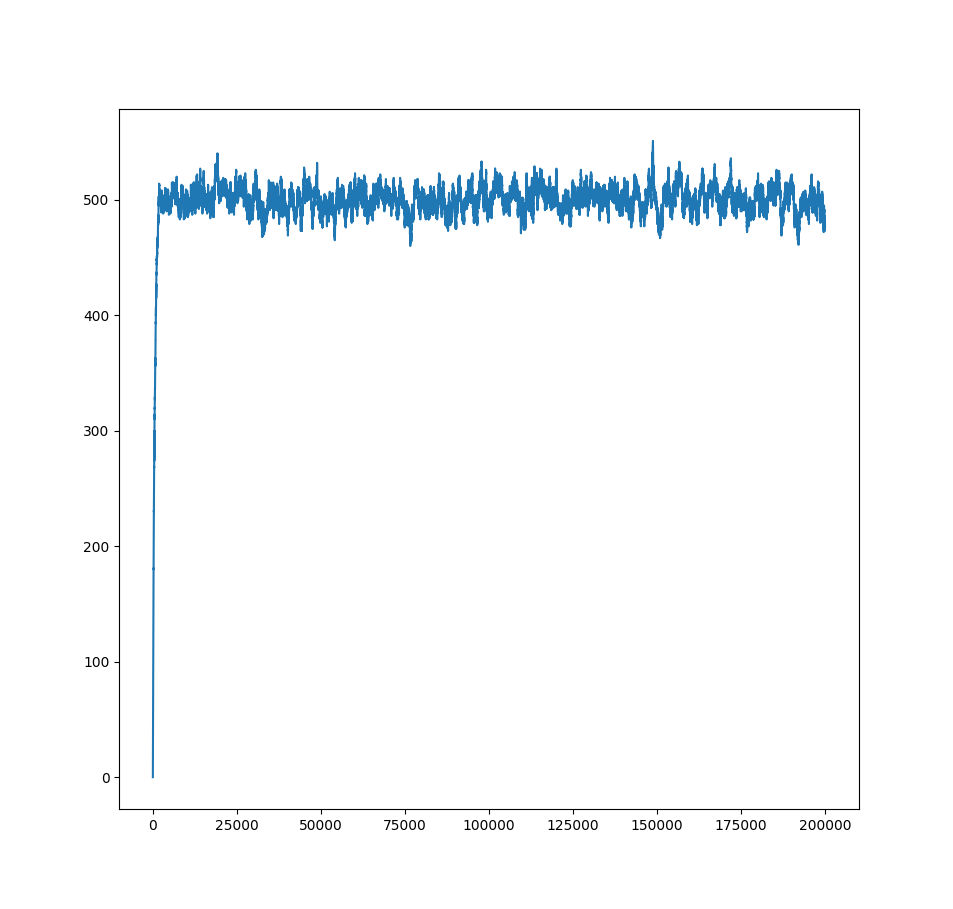
\includegraphics[width=0.8\textwidth]{q6a}
    \caption{Graph for $X_t$ in question 6.}
    \label{fig:q6a}
\end{figure}

\begin{figure}[htpb]
    \centering
    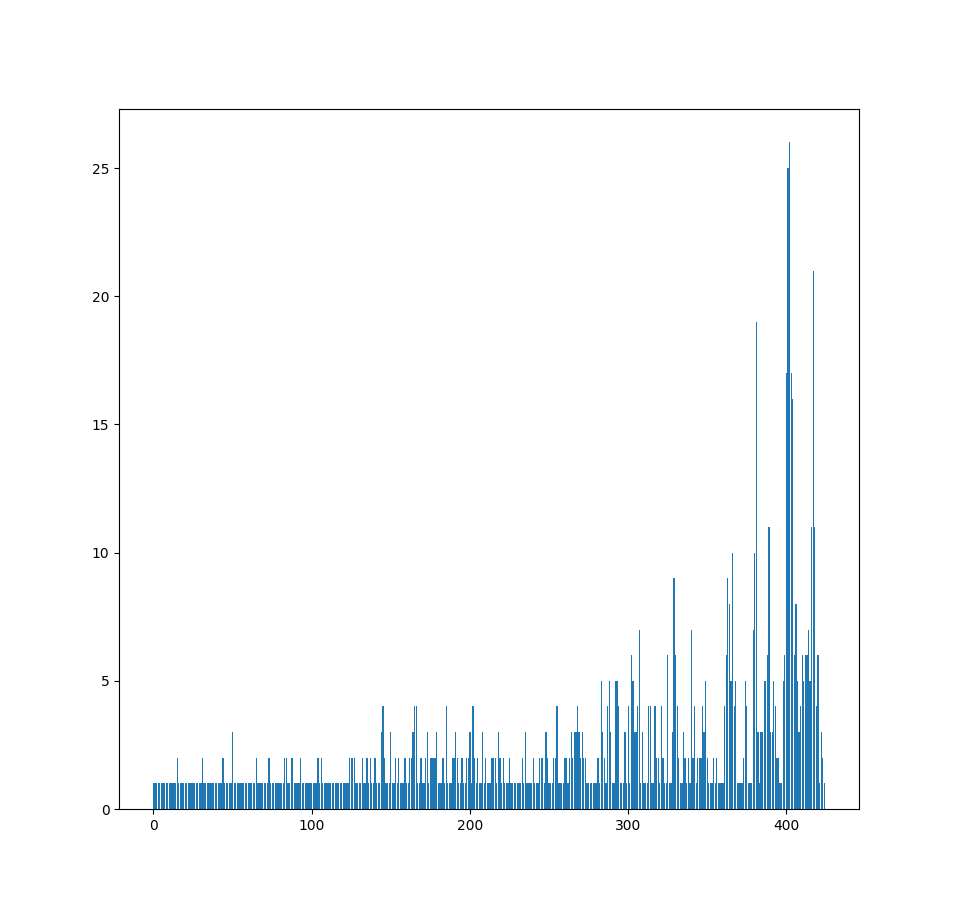
\includegraphics[width=0.8\textwidth]{q6b}
    \caption{Histogram of how many times each state was visited from time 0 to 1000}
    \label{fig:q6b}
\end{figure}

\begin{figure}[htpb]
    \centering
    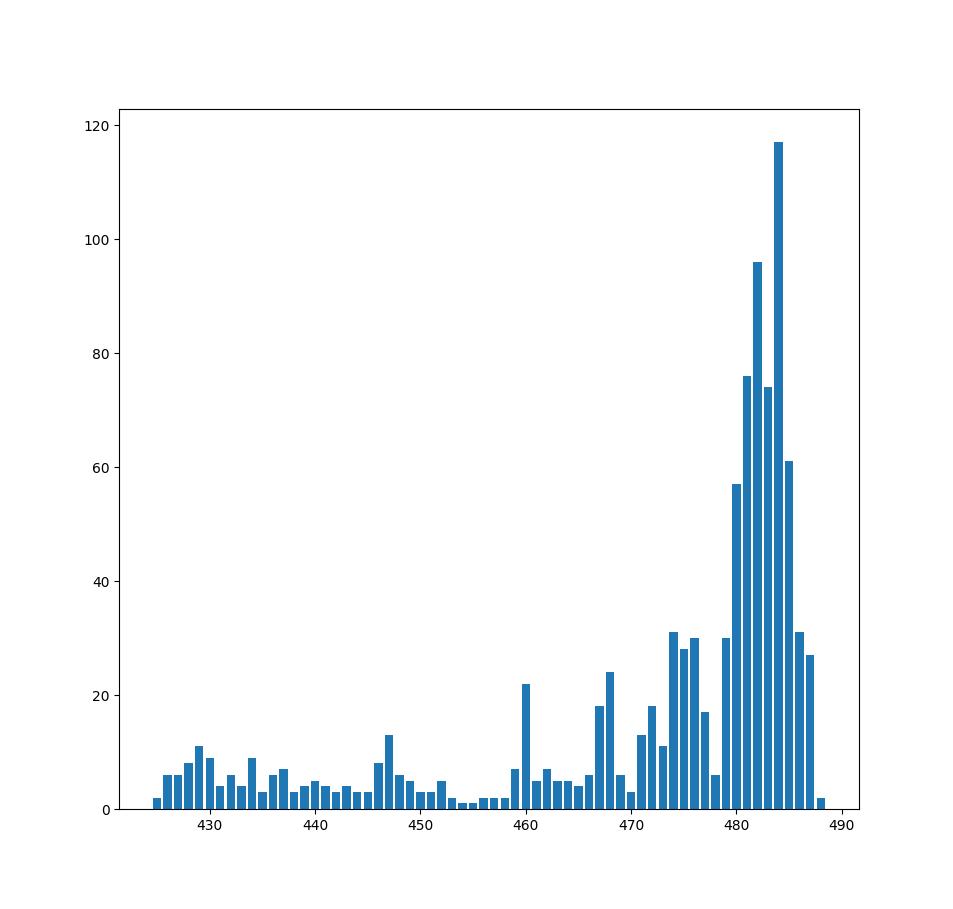
\includegraphics[width=0.8\textwidth]{q6c}
    \caption{Histogram of how many times each state was visited from time 1000 to 2000}
    \label{fig:q6c}
\end{figure}

\begin{figure}[htpb]
    \centering
    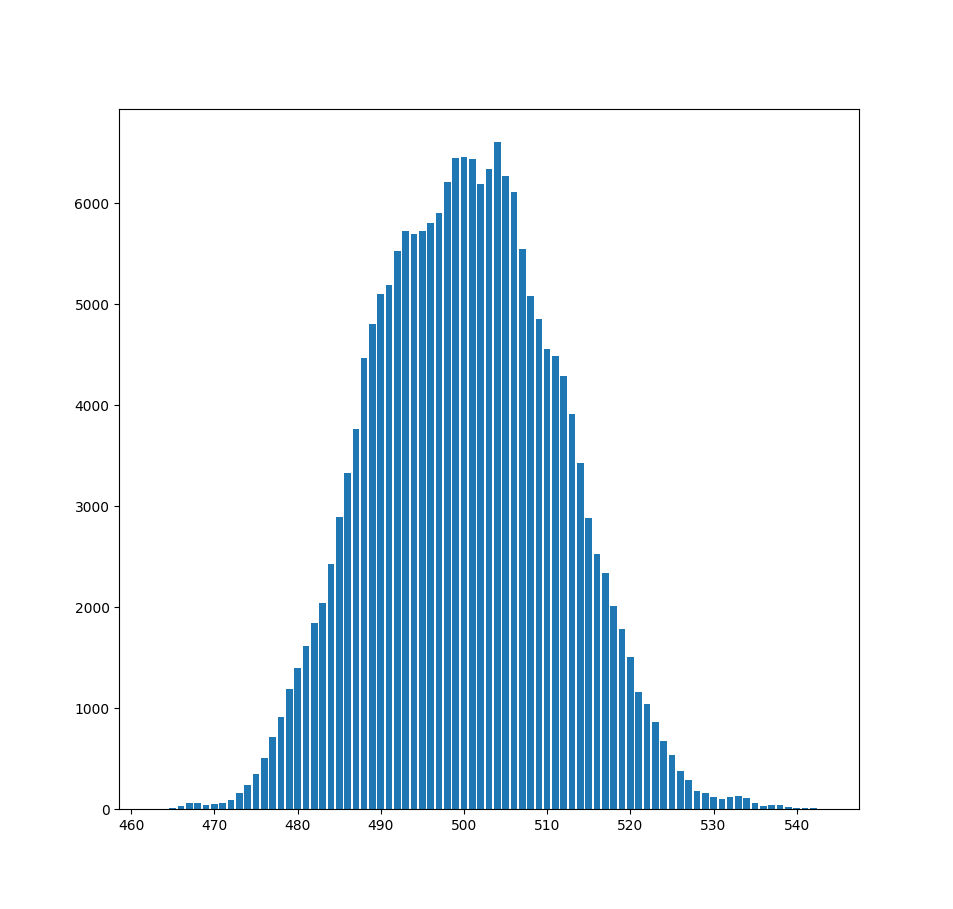
\includegraphics[width=0.8\textwidth]{q6d}
    \caption{Histogram of how many times each state was visited from time 10000 to 20000}
    \label{fig:q6d}
\end{figure}

\end{document}
